\chapter{Appendice}
In questa sezione verranno approfondite alcune funzioni di CPLEX necessarie ad implementare gli algoritmi descritti nei capitoli precedenti. Inoltre vengono analizzati tutti gli altri programmi, utilizzati nella stampa delle soluzioni e nell'analisi delle performance.

\section{CPLEX}
\subsection{Funzioni}
\subsubsection{Costruzione modello}
Per poter costruire il modello da analizzare, come prima cosa, è necessario creare un puntatore alle due strutture dati utilizzate da CPLEX.
\lstinputlisting[caption={\footnotesize{modelTSP.txt}}, style=code, firstnumber=1, firstline=27, lastline=29, label=tsp_model, language=c]{Source/modelTSP.txt}
La funzione alla riga 2 alloca la memoria necessaria e riempie la struttura con valori di default. Nel caso in cui non termini con successo memorizza un codice d'errore in \textit{\&error}.\\
La funziona invocata nella riga successiva, invece, associa la struttura LP all'ENV che gli viene fornito. Il terzo parametro passato, nell'esempio "TSP", sarà il nome del modello creato.
Al termine di queste operazioni verrà quindi creato un modello vuoto. All'interno del nostro programma per inizializzarlo è stata costruita la seguente funzione:
\begin{center}
\begin{tabular}{c}
\begin{lstlisting}[linewidth=320pt, basicstyle=\footnotesize\sffamily,] 
void cplex_build_model(istanza_problema, env , lv);
\end{lstlisting}
\end{tabular}
\end{center}
\begin{table}[h]
\centering
\begin{tabular}{rl}
\textbf{istanza\_problema: } & {puntatore alla struttura che contiene} \\
&  {l'istanza del problema (letta dal file TSPlib)} \\
\textbf{env: } & {puntatore di tipo CPXENVptr alla}\\
& {struttura ENV precedentemente creata}\\
\textbf{lp: } & {puntatore di tipo CPXLPptr alla}\\
& {struttura LP  precedentemente creata}\\
\end{tabular}
\end{table}
All'interno di \textbf{cplex\_build\_model()} viene aggiunta una colonna alla volta al modello, definendo quindi anche la funzione obiettivo. Le variabili aggiunte corrispondono agli archi del grafo e per ciascuno di questi viene calcolato il costo come distanza euclidea. La funzione necessaria ad inserire colonne e definire la funzione di costo è la seguente:
\vspace{0.5cm}
\begin{center}
\begin{tabular}{c}
\begin{lstlisting}[linewidth=350pt, basicstyle=\footnotesize\sffamily,]     
CPXnewcols(env, lp, num_colonne, costi, lower_bound, 
           upper_bound, tipi_variabili, nomi_variabili);
\end{lstlisting}
\end{tabular}
\end{center}
\begin{table}[h]
\begin{tabular}{rl}
\textbf{env:} & {puntatore di tipo CPXENVptr alla}\\
& {struttura ENV precedentemente creata} \\
\textbf{lp:} & {di tipo CPXLPptr, è un puntatore alla struttura LP}\\
& {precedentemente creata}\\
\textbf{num\_colonne:} & {numero di colonne da inserire} \\    
\textbf{costi:} & {vettore dei costi relativi agli archi da inserire} \\
\textbf{lower\_bound:} & {vettore contenente i lower bound dei valori}\\
& {assumibili dalle variabili da inserire}\\              
\textbf{upper\_bound:} & {vettore contenente gli upper bound dei valori}\\
&  {assumibili dalle variabili da inserire} \\
\textbf{tipi\_variabili:} & {vettore contenente la tipologia delle variabili}\\
& da inserire\\
\textbf{nomi\_variabili:} & {vettore di stringhe contenenti i nomi}\\
& {delle variabili da inserire}
\end{tabular}
\end{table}
La generica colonna \textbf{i}, aggiunta dalla funzione, sarà definita dalle informazioni contenute all'interno della posizione \textbf{i} degli array, ricevuti come parametri. Nel programma elaborato durante il corso, viene aggiunta una colonna alla volta all'interno del modello. Per far ciò, è necessario comunque utilizzare riferimenti alle informazioni da inserire, in modo da ovviare il problema riguardante la tipologia di argomenti richiesti, che sono array. Ad esempio, nel nostro caso, la tipologia di una nuova variabile inserita sarà un riferimento al carattere \textbf{'B'}, che la identifica come binaria.\\
Per poter inserire il primo insieme di vincoli del problema\\
$$
\underset{e\in \delta(v)}\sum{\;x_e} = 2\;\;\;\;\;\;\;\;\;\;\;\;\;\;\;\;\;\;\forall\;v\in V \\\\
$$
\\
viene invece sfruttata la seguente funzione:
\begin{center}
\begin{tabular}{c}
\begin{lstlisting}[linewidth=330pt, basicstyle=\footnotesize\sffamily,]     
 CPXnewrows(env, lp, numero_righe,termini_noti,
            tipi_vincoli, range_valori, nomi_vincoli);
\end{lstlisting}
\end{tabular}
\end{center}
\begin{table}[h]
\centering
\begin{tabular}{rl}
\textbf{env:} & {puntatore di tipo CPXENVptr alla struttura ENV}\\
& {precedentemente creata}\\
\textbf{lp:} & {puntatore di tipo CPXLPptr alla struttura LP}\\
& {precedentemente creata}\\
\textbf{numero\_righe:} & {numero di righe (vincoli) da inserire}\\
\textbf{termini\_noti:} & {vettore dei termini noti dei vincoli}\\
\textbf{tipi\_vincoli:} & {vettore di caratteri che specifica il tipo di vincoli}\\
&{da inserire. Ogni carattere può assumere:}\\
&{\textit{'L'} per vincolo $\leq$}\\
&{\textit{'E'} per vincolo $=$}\\
&{\textit{'G'} per vincolo $\geq$}\\
&{\textit{'R'} per vincolo definito in un intervallo}\\
\textbf{range\_valori:} & {vettore di range per i valori di ogni vincolo}\\
& {(nel nostro caso è NULL)} \\
\textbf{nomi\_vincoli} & vettore di stringhe contenenti i nomi  \\
                  & delle variabili da inserire
\end{tabular}
\end{table}
In modo analogo all'inserimento delle colonne, nel nostro programma viene aggiunta una riga alla volta nel modello. L'\textbf{i}-esima riga aggiunta corrisponderà al vincolo imposto sul nodo \textbf{i}-esimo, imponendo a 1 il coefficiente della variabile $x_{k,j}$ se $k=i$ $j=i$ per ogni variabile del modello. In questo modo però viene aggiunto un vincolo in cui è necessario cambiare i coefficienti delle variabili che ne prendono parte. Per fare ciò è necessaria la funzione:
\begin{center}
\begin{tabular}{c}
\begin{lstlisting}[linewidth=230pt, basicstyle=\footnotesize\sffamily,]     
CPXchgcoef(env, lp, i, j, new_value);
\end{lstlisting}
\end{tabular}
\end{center}
\begin{table}[h]
\centering
\begin{tabular}{rl}
\textbf{env:} & {puntatore di tipo CPXENVptr alla struttura ENV}\\
& {precedentemente creata}\\
\textbf{lp:} & {puntatore di tipo CPXLPptr alla struttura LP}\\
& {precedentemente creata}\\
\textbf{i:} & {intero che specifica l'indice della riga in cui modificare il }\\
&{coefficiente}\\
\textbf{j:} & {intero che specifica la colonna in cui si trova la variabile}\\
&{di cui modificare il coefficiente}\\
\textbf{new\_value:} & {nuovo valore del coefficiente}\\
\end{tabular}
\end{table}
L'utilizzo di questa metodo per inserire nuovi vincoli è però considerato inefficiente. Al suo posto è consigliato l'utilizzo di una funzione che inserisca il vincolo con già i coefficienti delle variabili impostati al valore corretto:
\begin{center}
\begin{tabular}{c}
\begin{lstlisting}[linewidth=385pt, basicstyle=\footnotesize\sffamily,]     
CPXaddrows(env, lp, num_nc, num_nr, nnz, const_term, type_costr,
           rmatbeg, rmatind, rmatval, col_name, row_name);
\end{lstlisting}
\end{tabular}
\end{center}
\begin{table}[h]
\centering
\begin{tabular}{rl}
\textbf{env:} & {puntatore di tipo CPXENVptr alla struttura ENV}\\
& {precedentemente creata}\\
\textbf{lp:} & {puntatore di tipo CPXLPptr alla struttura LP}\\
& {precedentemente creata}\\
\textbf{num\_nc:} & {numero di nuove colonne che devono essere aggiunte}\\
\textbf{num\_nr:} & {numero di nuove righe che devono essere aggiunte}\\
\end{tabular}
\end{table}
\begin{table}[h]
\centering
\begin{tabular}{rl}
\textbf{nnz:} & {numero di coefficienti non nulli nel vincolo aggiunto}\\
\textbf{const\_term:} & {vettore con i termini noti per ogni vincolo da aggiungere}\\
\textbf{type\_costr:} & {vettore con il tipo di vincoli da aggiungere,}\\
&{scelto tra:}\\
&{\textit{'L'} per vincolo $\leq$}\\
&{\textit{'E'} per vincolo $=$}\\
&{\textit{'G'} per vincolo $\geq$}\\
&{\textit{'R'} per vincolo definito in un intervallo}\\
\textbf{rmatbeg:} & {vettore per definire le righe da aggiungere}\\
\textbf{rmatind:} & {vettore per definire le righe da aggiungere}\\
\textbf{rmatval:} & {vettore per definire le righe da aggiungere}\\
\textbf{col\_name:} & {vettore contenente i nomi delle nuove colonne}\\
\textbf{row\_name:} & {vettore contenente i nomi dei nuovi vincoli}\\
\end{tabular}
\end{table}
 
\subsubsection{Calcolo della soluzione}
Per ottenere la soluzione ottima del problema di ottimizzazione del problema correlato al modello definito in cplex, vengono utilizzate due fasi:
\begin{itemize}
\item{\textbf{Risoluzione del problema di ottimizzazione}\\
\begin{center}
\begin{tabular}{c}
\begin{lstlisting}[linewidth=120pt, basicstyle=\footnotesize\sffamily,]
CPXmipopt(env, lp);
\end{lstlisting}
\end{tabular}
\end{center}
\begin{table}[h]
\centering
\begin{tabular}{rl}
\textbf{env:} & {puntatore di tipo CPXENVptr alla struttura ENV}\\
& {precedentemente creata}\\
\textbf{lp:} & {puntatore di tipo CPXLPptr alla struttura LP}\\
& {precedentemente creata}\\
\end{tabular}
\end{table}
}
\item{\textbf{Ottenimento della soluzione}\\
\begin{center}
\begin{tabular}{c}
\begin{lstlisting}[linewidth=230pt, basicstyle=\footnotesize\sffamily,]
CPXgetx(env, lp, x, inizio, fine);
\end{lstlisting}
\end{tabular}
\end{center}
\begin{table}[h]
\centering
\begin{tabular}{rl}
\textbf{env:} & {puntatore di tipo CPXENVptr alla struttura ENV}\\
& {precedentemente creata}\\
\textbf{lp:} & {puntatore di tipo CPXLPptr alla struttura LP}\\
& {precedentemente creata}\\
\textbf{x:} & {puntatore a un vettore di double in cui verranno salvati}\\
\end{tabular}
\end{table}
\begin{table}[h]
\centering
\begin{tabular}{rl}
& {i valori delle variabili ottenuti dalla soluzione ottima}\\
\textbf{inizio:} & {primo indice della variabile di cui si vuole memorizzare}\\
& {ed analizzare il valore}\\
\textbf{fine:} & {indice dell'ultima variabile di cui si vuole memorizzare}\\
& {ed analizzare il valore}\\
\end{tabular}
\end{table}
Questa funzione salva in x tutte le variabili che hanno indice $i\in [inizio, fine]$ e quindi x deve essere un vettore di almeno $fine-inizio+1$ valori. Nel nostro programma, vengono analizzati i valori di tutte le variabili in gioco.\\
Per questo motivo \textbf{inizio=0} e \textbf{fine=num\_colonne - 1}\footnote{numero di variabili=CPXgetnumcols(env,lp);}\footnote{numero di vincoli=CPXgetnumrows(env,lp);}. In seguito il nostro programma analizza la correttezza della soluzione svolgendo la verifica su:
\begin{itemize}
\item{\textit{valori assunti dalle variabili}\\
ciascun $x_{i,j}$ assume valore $0$ o $1$ con una tolleranza di $\epsilon=10^{-5}$}
\item{\textit{grado di ciascun nodo}\\
il tour è composto al massimo da due archi che toccano lo stesso nodo}
\end{itemize}
}
\end{itemize}
\subsubsection{Lazy constraints}
Nel caso in cui si voglia sfruttare la possibilità di verificare se è stato rispettato un vincolo, solo al termine della computazione della soluzione, è necessario inserire un "lazy constraint". Per fare ciò viene utilizzata la seguente funzione:
\begin{center}
\begin{tabular}{c}
\begin{lstlisting}[linewidth=380pt, basicstyle=\footnotesize\sffamily,]     
CPXaddlazyconstraints(env, lp, num_vincoli, nnz, 
					termine_costante, tipo_vincolo, posizione_iniziale,
					indici, valori, nome_vincolo);
\end{lstlisting}
\end{tabular}
\end{center}
\begin{table}[h]
\centering
\begin{tabular}{rl}
\textbf{env:} & {puntatore di tipo CPXENVptr alla struttura ENV}\\
& {precedentemente creata}\\
\textbf{lp:} & {puntatore di tipo CPXLPptr alla struttura LP}\\
& {precedentemente creata}\\
\textbf{num\_vincoli:} & {numero di vincoli da inserire}\\
\textbf{nnz:} & {vettore con il numeri di variabili per ogni vincolo}\\ 
\end{tabular}
\end{table}
\begin{table}[h]
\centering
\begin{tabular}{rl}
\textbf{termine\_costante:} & {vettore dei termini noti dei vincoli}\\
\textbf{tipi\_vincoli:} & {vettore di caratteri che specifica il tipo di vincoli}\\
&{da inserire. Ogni carattere può assumere:}\\
&{\textit{'L'} per vincolo $\leq$}\\
&{\textit{'E'} per vincolo $=$}\\
&{\textit{'G'} per vincolo $\geq$}\\
&{\textit{'R'} per vincolo definito in un intervallo}\\
\textbf{posizione\_iniziale:} & {vettore con le posizione iniziali dei coefficienti nei}\\
&{vincoli}\\
\textbf{indici:} & {vettore di vettori contenenti gli indici delle}\\
& {variabili appartenenti al vincolo}\\
\textbf{valori:} & {vettore di vettori con i coefficienti delle variabili del vincolo}\\
\textbf{nome\_vincolo:} & {vettore con i nomi}\\
& {dei vincoli}\\
\end{tabular}
\end{table}
In modo analogo alle due funzioni precedentemente descritte per l'aggiunta di righe e colonne, nel nostro modello viene inserito un vincolo per volta. Per impostare correttamente i coefficienti delle variabili presenti nel vincolo, vengono sfruttati i due array \textit{indici} e \textit{valori}. Come rappresentato in Figura \ref{lazy_constraints}, all'interno della posizione \textit{i}-esima del vettore di indici è presente la posizione dell'\textit{i}-esima variabile del vincolo da inserire (nell'esempio in figura $indici[i]=j$). Mentre l'\textit{i}-esima posizione del vettore di valori contiene il corrispondente  coefficiente (in questo caso $c_j$).
\begin{figure}[h] 
\begin{center} 
  % Requires \usepackage{graphicx} 
  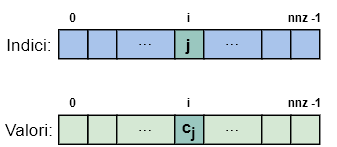
\includegraphics[scale=0.5]{Images/lazy_constraints} 
  \caption{\footnotesize{Array lazy constraints}}
  \label{lazy_constraints} 
\end{center} 
\end{figure}
\vspace{10cm}
\subsubsection{Lazy Constraint Callback}
Per poter utilizzare una lazy constraint callback, precedentemente implementata, all'interno del programma, prima di tutto è necessario installarla. Questo viene fatto attraverso la seguente funzione:
\begin{center}
\begin{tabular}{c}
\begin{lstlisting}[linewidth=380pt, basicstyle=\footnotesize\sffamily,]     
CPXsetlazyconstraintcallbackfunc(env, mylazycallback, tsp_in);
\end{lstlisting}
\end{tabular}
\end{center}
\begin{table}[h]
\centering
\begin{tabular}{rl}
\textbf{env:} & {puntatore di tipo CPXENVptr alla struttura ENV}\\
\textbf{mylazycallback:} & {puntatore di tipo CPXPUBLIC * alla callback chiamata}\\
\textbf{tsp\_in:} & {puntatore di tipo void* ad una struttura dati }\\
& {contenente le informazioni da passare alla callback}\\
\end{tabular}
\end{table}
Una volta installata la callback è necessario cambiare l'impostazione del numero di thread utilizzati dal programma. Infatti CPLEX, non sapendo se la funzione implementata dall'utente è thread safe, impedisce lo svolgimento di elaborazioni in parallelo con le callback. A meno che questo non venga esplicitamente dichiarato dall'utente con l'impostazione del corrispondente parametro.
Per questo può tornare utile la seguente funzione, che restituisce il numero di core presenti nel computer:\\
\begin{center}
\begin{tabular}{c}
\begin{lstlisting}[linewidth=170pt, basicstyle=\footnotesize\sffamily,]
CPXgetnumcores(env, ncores); 
\end{lstlisting}
\end{tabular}
\end{center}
\begin{table}[h]
\centering
\begin{tabular}{rl}
\textbf{env:} & {puntatore di tipo CPXENVptr ad una struttura ENV}\\
\textbf{ncores:} & {puntatore alla variabile in cui viene scritto il numero di core}\\            
\end{tabular}
\end{table} 
Come descritto nella sezione dedicata, le callback sono funzioni lasciate appositamente vuote da CPLEX, affinché l'utente possa implementarle in maniera personalizzata. Hanno però una dichiarazione standard, qui riportata: 
\begin{center}
\begin{lstlisting}[linewidth=380pt, basicstyle=\footnotesize\sffamily,]     
static int CPXPUBLIC name_function(CPXCENVptr env, void* cbdata, 
								   								int wherefrom, void* cbhandle, 	
								   								int* useraction_p)
\end{lstlisting}
\end{center}
\vspace{2cm}
\begin{table}[h]
\centering
\begin{tabular}{rl}
\textbf{env:} & {puntatore di tipo CPXENVptr ad una struttura ENV}\\
\textbf{cbdata:} & {puntatore che contiene specifiche informazioni per la}\\
&{callback}\\
\textbf{wherefrom:} & {contiene dove è stata invocata la callback durante} \\ 
&{l'ottimizzazione}\\
\textbf{cbhandle:} & {puntatore a dati privati dell'utente} \\
\textbf{useraction\_p:} & {specifica le azioni da eseguire al termine della callback:}\\
& {CPX\_CALLBACK\_DEFAULT: usa il nodo di CPLEX}\\
&{selezionato}\\
& {CPX\_CALLBACK\_FAIL: esci dell'ottimizzazione}\\
& {CPX\_CALLBACK\_SET: usa il nodo selezionato come}\\  
& {definito nel valore di ritorno}\\            
\end{tabular}
\end{table} 
Nell'implementarla bisogna fare particolare attenzione a renderla thread safe, se si vuole utilizzarla su più processi in parallelo. Infatti, nel caso in cui il programma lavorasse contemporaneamente con più processori, non si devono verificare interferenze di accesso agli stessi dati da parte di invocazioni diverse della callback. Quest'aspetto è lasciato a completa gestione dell'utente.\\
%CONTROLLARE COSA VUOL DIRE CPXPUBLIC
Per avere accesso alle variabili utilizzate dal nodo che invoca la callback è possibile chiamare la seguente funzione:
\begin{center}
\begin{tabular}{c}
\begin{lstlisting}[linewidth=380pt, basicstyle=\footnotesize\sffamily,]     
CPXgetcallbacknodex(env, cbdata, wherefrom, x_star, start, end);
\end{lstlisting}
\end{tabular}
\end{center}
\begin{table}[h]
\centering
\begin{tabular}{rl}
\textbf{env:} & {puntatore di tipo CPXENVptr ad una struttura ENV}\\
\textbf{cbdata:} & {puntatore che contiene specifiche informazioni per la callback}\\
\textbf{wherefrom:} & {contiene in che punto dell'ottimizzazione è stata invocata la} \\ 
&{callback}\\
\textbf{x\_star:} & {vettore in cui memorizzare le variabili} \\
\textbf{begin} & {indice della prima variabile che si vuole venga restituita}\\
\textbf{end} & {indice dell'ultima variabile che si vuole venga restituita}\\           
\end{tabular}
\end{table}
Invece, per ottenere informazioni riguardanti il problema di ottimizzazione che si sta risolvendo all'interno di una callback implementata dall'utente, è possibile utilizzare:
\begin{center}
\begin{tabular}{c}
\begin{lstlisting}[linewidth=380pt, basicstyle=\footnotesize\sffamily,]  
CPXgetcallbackinfo(env, cbdata, wherefrom, which_info, result);
\end{lstlisting}
\end{tabular}
\end{center}
\begin{table}[h]
\centering
\begin{tabular}{rl}
\textbf{env:} & {puntatore di tipo CPXENVptr ad una struttura ENV}\\
\textbf{cbdata:} & {puntatore che contiene specifiche informazioni per la callback}\\
\textbf{wherefrom:} & {contiene in che punto dell'ottimizzazione è stata invocata la}\\ 
&{callback}\\
\textbf{which\_info:} & {macro che specifica l'informazione che si desidera conoscere} \\
\textbf{result:} & {puntatore di tipo void in cui verrà memorizzata}\\          
&{l'informazione richiesta}\\
\end{tabular}
\end{table}
Macro utili da utilizzare come parametro \textit{which\_info} possono essere:
\begin{table}[h]
\centering \footnotesize
\begin{tabular}{|r|l|}
\hline
\textbf{CPX\_CALLBACK\_INFO\_MY\_THREAD\_NUM:} & {identifica il thread che }\\
&{ha eseguito la chiamata}\\
\hline
\textbf{CPX\_CALLBACK\_INFO\_BEST\_INTEGER:} & {valore della miglior}\\
&{soluzione intera}\\
\hline
\end{tabular}
\end{table}
\\Per conoscere il valore della funzione obiettivo del problema legato al nodo corrente che invoca la callback:
\begin{center}
\begin{tabular}{c}
\begin{lstlisting}[linewidth=340pt, basicstyle=\footnotesize\sffamily,]  
CPXgetcallbacknodeobjval(env, cbdata, wherefrom, objval);
\end{lstlisting}
\end{tabular}
\end{center}
\begin{table}[h]
\centering
\begin{tabular}{rl}
\textbf{env:} & {puntatore di tipo CPXENVptr ad una struttura ENV}\\
\textbf{cbdata:} & {puntatore che contiene specifiche informazioni per la callback}\\
\textbf{wherefrom:} & {contiene in che punto dell'ottimizzazione è stata invocata la} \\ 
&{callback}\\
\textbf{objval:} & {puntatore ad una variabile \textit{double} in cui memorizzare il costo} \\
\end{tabular}
\end{table}
All'interno della lazy callback è necessario aggiungere il taglio voluto al nodo corrente che la invoca, per questo viene chiamata la funzione, che ne aggiunge uno alla volta:
\begin{center}
\begin{tabular}{c}
\begin{lstlisting}[linewidth=350pt, basicstyle=\footnotesize\sffamily,]  
CPXcutcallbackadd(env, cbdata, wherefrom, nnz, const_term, 
                   type_constraint, indices, values, 
                   purgeable);
\end{lstlisting}
\end{tabular}
\end{center}
\begin{table}[h]
\centering
\begin{tabular}{rl}
\textbf{env:} & {puntatore di tipo CPXENVptr ad una struttura ENV}\\
\textbf{cbdata:} & {puntatore che contiene specifiche informazioni per la}\\
&{callback}\\
\textbf{wherefrom:} & {contiene in che punto dell'ottimizzazione è stata} \\ 
&{invocata la callback}\\
\textbf{nnz:} & {numero di coefficienti non nulli} \\
\textbf{const\_term:} & {valore del termine noto} \\
\textbf{type\_constraint:} & {tipologia del taglio da aggiungere, a scelta tra} \\
&{\textit{'L'} per vincolo $\leq$}\\
&{\textit{'E'} per vincolo $=$}\\
&{\textit{'G'} per vincolo $\geq$}\\
\textbf{indices:} & {vettore contente gli indici dei coefficienti del taglio} \\
\textbf{values:} & {vettore contenente i coefficienti delle variabili nel} \\
&{taglio}\\
\textbf{purgeable:} & {intero che specifica in che modo CPLEX deve } \\
&{trattare il taglio, consigliato 0}\\
\end{tabular}
\end{table}
In questo modo il taglio aggiunto risulta essere globale, se si vuole aggiungere un taglio visibile solo localmente, cioè solo per i nodi discendenti a quello che invoca la callback, è necessaria òa chiamata:
\begin{center}
\begin{tabular}{c}
\begin{lstlisting}[linewidth=380pt, basicstyle=\footnotesize\sffamily,]  
CPXcutcallbackaddlocal(env, cbdata, wherefrom, nnz, const_term,
                       type_constraint, indices, values);
\end{lstlisting}
\end{tabular}
\end{center}
\begin{table}[h]
\centering
\begin{tabular}{rl}
\textbf{env:} & {puntatore di tipo CPXENVptr ad una struttura ENV}\\
\textbf{cbdata:} & {puntatore che contiene specifiche informazioni per la callback}\\
\textbf{wherefrom:} & {contiene in che punto dell'ottimizzazione è stata invocata la} \\ 
\end{tabular}
\end{table}
\begin{table}[h]
\centering
\begin{tabular}{rl}
&{callback}\\
\textbf{nnz:} & {numero di coefficienti non nulli} \\
\textbf{const\_term:} & {valore del termine noto} \\
\textbf{type\_constraint:} & {tipologia del taglio da aggiungere, a scelta tra} \\
&{\textit{'L'} per vincolo $\leq$}\\
&{\textit{'E'} per vincolo $=$}\\
&{\textit{'G'} per vincolo $\geq$}\\
\textbf{indices:} & {vettore contente gli indici dei coefficienti del taglio} \\
\textbf{values:} & {vettore contenente i coefficienti delle variabili nel} \\
&{taglio}\\
\end{tabular}
\end{table}

\subsection{Parametri}\label{param}
Con le seguenti funzioni è possibile modificare i parametri di impostazione di CPLEX, altrimenti impostati ai valori di default.
Nel caso in cui si tratti di parametri di tipo INT è necessario invocare:\\
\begin{center}
\begin{tabular}{c}
\begin{lstlisting}[linewidth=330pt, basicstyle=\footnotesize\sffamily,]     
CPXsetintparam(env, numero_parametro, nuovo_valore);
\end{lstlisting}
\end{tabular}
\end{center}
mentre se di tipo DOUBLE:\\
\begin{center}
\begin{tabular}{c}
\begin{lstlisting}[linewidth=330pt, basicstyle=\footnotesize\sffamily,]     
CPXsetdblparam(env, numero_parametro, nuovo_valore);
\end{lstlisting}
\end{tabular}
\end{center}
In entrambe le funzioni:
\begin{table}[h]
\centering
\begin{tabular}{rl}
\textbf{env:} & {puntatore di tipo CPXENVptr alla struttura ENV}\\
& {di cui si vogliono cambiare i parametri}\\
\textbf{numero\_parametro:} & {intero corrispondente al parametro da modificare}\\
& {(vedi Tabella \ref{param_table})}\\
\textbf{nuovo\_valore:} & {nuovo valore (rispettivamente intero o double)}\\
& {del parametro}\\
\end{tabular}
\end{table}

\begin{table}[h]
\centering\footnotesize
\begin{tabular}{|l|l|}
\hline
\multirow{3}{*}{\textbf{CPX\_PARAM\_EPGAP}} & {tolleranza dell'intervalo tra la migliore funzione }\\
& {obiettivo intera e la funzione obiettivo del}\\
& {miglior nodo rimanente.}\\
\hline
\multirow{3}{*}{\textbf{CPX\_PARAM\_NODELIM}} & {massimo numero di nodi da risolvere prima}\\
& {che l'algoritmo termini senza aver aggiunto l'ottimalità}\\
& {(0 impone di fermarsi alla radice).}\\
\hline
\multirow{3}{*}{\textbf{CPX\_PARAM\_POPULATELIM}} & {limita il numero di soluzioni MIP generate }\\
& {per il pool di soluzioni durante ogni chiamata alla}\\
&{procedura populate.}\\
\hline
\textbf{CPX\_PARAM\_SCRIND} & {visione o meno dei messaggi di log di CPLEX}\\
\hline
\textbf{CPX\_PARAM\_MIPCBREDLP} & {permette, dalla callback chiamata, di accedere  }\\
&{al modello originale del problema e non a quello ridotto .}\\
\hline
\textbf{CPX\_PARAM\_THREADS} & {imposta il numero massimo di thread utilizzabili. }\\
\hline
\end{tabular}
\caption{Parametri.}\label{param_table}
\end{table}
\subsection{Costanti utili}
Di seguito sono riportate alcune macro utili di CPLEX, insieme ai loro corrispondenti valori:
\begin{table}[h]
\footnotesize\centering
\begin{tabular}{|r|l|}
\hline
\textbf{CPX\_ON} & {\textbf{1}}\\
{} & {valore da assegnare ad alcuni parametri per abilitarli}\\
\hline
\textbf{CPX\_OFF} & {0}\\
{} & {valore da assegnare ad alcuni parametri per disabilitarli}\\
\hline
\textbf{CPX\_INFBOUND} & {$+\infty$}\\
{} & {massimo valore intero utilizzabile in CPLEX}\\
\hline
\end{tabular}
\end{table}

\section{Gnuplot}\label{gnuplot}
Una volta ottenuta la soluzione del problema di ottimizzazione, viene disegnato il grafo per facilitare all'utente la comprensione della sua correttezza. Per fare ciò viene utilizzato Gnuplot, un programma di tipo command-driven.\\
Per poterlo utilizzare all'interno del proprio programma esistono due metodi:
\begin{itemize}
\item{Collegare la libreria ed invocare le sue funzioni all'interno del nostro programma}
\item{Collegare l'eseguibile interattivo al proprio programma. In questo caso i comandi deve essere passati all'eseguibile attraverso un file di testo e l'utilizzo di un pipe.}\\
\end{itemize}
In questa trattazione è stato scelto il secondo metodo. All'interno del file è possibile specificare a Gnuplot le caratteristiche grafiche che deve aver il grafo. Di seguito viene riportato un esempio di tale file.\\

\lstinputlisting[caption={\footnotesize{style.txt}}, style=code, firstnumber=1, firstline=1, lastline=12, label=style_example]{Source/style_example.txt}

Nell'esempio sopra riportato, nella prima parte viene definito lo stile, il colore delle linee e la tipologia di punti, che verrano in seguito visualizzati all'interno del grafico prodotto.\\In seguito viene effettuato il plot del grafo in una finestra, utilizzando il primo e secondo valore di ciascuna riga del file \textbf{solution.dat} come coordinate mentre il terzo valore viene utilizzato come etichetta.\\\\
Il file \textbf{solution.dat} contiene le informazioni relative alla soluzione del grafico in cui ciascuna riga ha la seguente forma:
\begin{center}
\begin{tabular}{c}
\begin{lstlisting}[linewidth=290pt,basicstyle=\footnotesize\sffamily,]     
coordinata_x   coordinata_y   posizione_in_tour
\end{lstlisting}
\end{tabular}
\end{center}
\textbf{coordinata\_x} rappresenta la coordinata x del nodo;\\
\textbf{posizione\_in\_tour} rappresenta la coordinata y del nodo;\\
\textbf{posizione\_in\_tour} rappresenta l'ordine del nodo all'interno del tour, assunto come nodo di origine il nodo 1.\\\\
Il grafico viene generato dal comando \textbf{plot}, leggendo tutte le righe non vuote e disegnando un punto nella posizione \textbf{(coordinata\_x,coordinata\_y)} del grafico 2D. In seguito viene tracciata una linea solo tra coppie di punti, legati a righe consecutive non vuote all'interno di \textbf{solution.dat}.\\\\
Attraverso le istruzioni riportate nelle righe 10-12 di \textbf{style.txt}, viene invece salvato il grafico appena generato nell'immagine \textbf{solution.png}.\\\\
Di seguito vengono riportate le varie fasi necessarie alla definizione di un pipe e al passaggio di questo al programma GNUplot:
\begin{itemize}
\item{\textbf{Definizione del pipe}
\lstinputlisting[style=code, firstnumber=1, firstline=1, lastline=1, label=style_example language=C]{Source/gnuplotC.txt}
dove \textbf{GNUPLOT\_EXE} è una stringa composta dal percorso completo dell'eseguibile di GNUplot, seguita dall'argomento \textbf{-persistent} (es. \textit{"D:/Programs/GNUplot/bin/gnuplot -persistent"}).
}
\item{\textbf{Passaggio delle istruzioni a GNUplot}
\lstinputlisting[style=code, firstnumber=2, firstline=2, lastline=10, label=style_example, language=C]{Source/gnuplotC.txt}
viene passata una riga alla volta, del file \textbf{style.txt}, a GNUplot mediante il pipe precedentemente creato.
}
\item{\textbf{Chiusura del pipe}
\lstinputlisting[style=code, firstnumber=11, firstline=11, lastline=11, label=style_example, language=C]{Source/gnuplotC.txt}
}
\end{itemize}

\section{perprof.py}\label{perf_profile_py}
Il programma utilizzato per la creazione del performance profile dei diversi algoritmo è perprof.py\cite{salvagnin_perf}. Di seuito vengono riportati i principali argomenti da linea di comando che possono essere utilizzati:

\begin{table}[h]
\begin{tabular}{|r|l|}
\hline
\textbf{-D delimiter} & {spefica che delimiter verrà usato come separatore tra le}\\
& {parole in una riga}\\
\hline
\textbf{-M value} & {imposta value come il massimo valore di ratio (asse x)}\\
\hline
\textbf{-S value} & {value rappresenta la quantità che viene sommata a}\\
& {ciascun tempo di esecuzione prima del confronto.}\\
& {Questo parametro è utile per non enfatizzare troppo}\\
& {le differenze di pochi ms tra gli algoritmi.}\\
\hline
\textbf{-L} & {stampa in scala logaritmica}\\
\hline
\textbf{-T value} & {nel file passato al programma, il TIME LIMIT=value}\\
\hline
\textbf{-P "title"} & {title è il titolo del plot}\\
\hline
\textbf{-X value} & {nome dell'asse x (default='Time Ratio')}\\
\hline
\textbf{-B} & {plot in bianco e nero}\\
\hline
\end{tabular}
\end{table}
Di seguito viene riportato un esempio dell'esecuzione del programma, del suo input e del suo output:
\begin{itemize}
\item{\textbf{comando}
\begin{center}
\begin{tabular}{c}
\begin{lstlisting}[linewidth=330pt, basicstyle=\footnotesize\sffamily,] 
python perfprof.py -D , -T 3600 -S 2 -M 20 esempio.csv
             out.pdf -P "all instances, shift 2 sec.s"
\end{lstlisting}
\end{tabular}
\end{center}
}
\item{\textbf{file di input con i dati}\\
Viene riportato parte del contenuto di esempio.csv .
\begin{center}
\begin{tabular}{c}
\begin{lstlisting}[linewidth=240pt, basicstyle=\footnotesize\sffamily,] 
3, Alg1, Alg2, Alg3
model_1.lp, 2.696693, 3.272468, 2.434147
model_2.lp, 0.407689, 1.631921, 1.198957
model_3.lp, 0.333669, 0.432553, 0.966638
\end{lstlisting}
\end{tabular}
\end{center}
La prima riga deve necessariamente contenere in ordine il numero di algoritmi analizzati e i loro nomi. Nelle righe seguenti viene riportato invece il nome del file lp e i tempi di esecuzione elencati secondo la sequenza di algortimti specificata all'inizio.
Ogni campo di ciascuna riga deve essere separato dal delimitatore specificato all'avvio del programma attraverso l'opzione -D.
}
\item{\textbf{immagine di output}\\
Il grafico viene restituito nel file out.pdf specificato da line di comando chiamando il programma.
\begin{figure}[h] 
\begin{center} 
  % Requires \usepackage{graphicx} 
  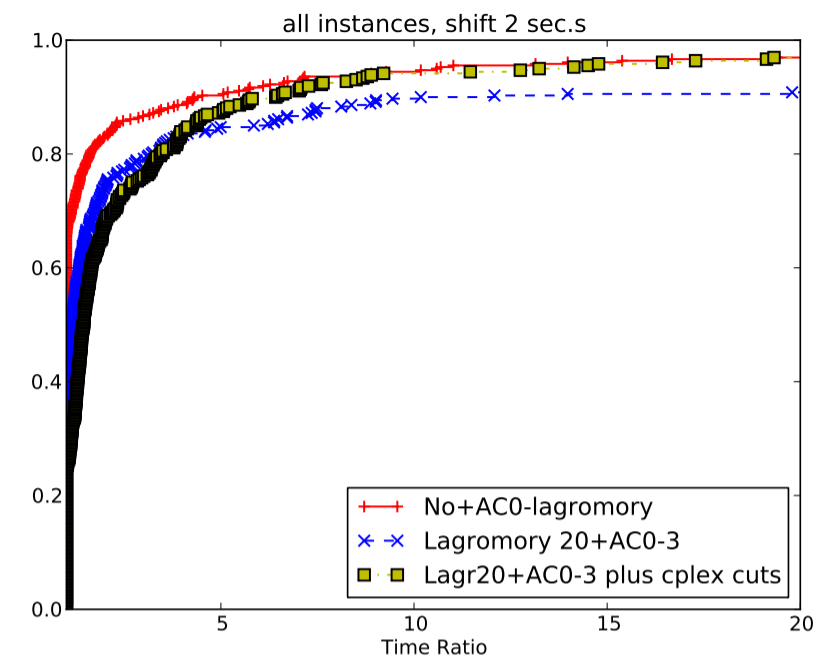
\includegraphics[scale=0.6]{Images/profile_out}\\ 
\end{center} 
\end{figure}
}
\end{itemize}
